\documentclass{report}
\usepackage[a4paper, margin=0.5in]{geometry}
\usepackage{parskip}
\usepackage{graphicx}
\usepackage{caption}
\usepackage{amssymb}
\usepackage{amsmath}
\usepackage{algpseudocode}
\usepackage{algorithm}

\captionsetup[figure]{
  font = it,
  labelfont = bf
}

\begin{document}
\begin{minipage}[b]{0.48\textwidth}
  \section*{K-Means Clustering}
  A clustering algorithm is an algorithm designed with the purpose of grouping, into an arbitrary number of classes, a set of points. Such classes are created by to grouping together those points that have common features. Thus, the goal of this category of algorithms is to build knowledge about the data provided as input that makes it possible to find hidden relationships among them which can be used to classify (into one of the classes created in the training stages) a point whose class is not known a priori.

  \section*{Standard (or Lloyd) Algorithm}
  In this section, the standard algorithm for implementing k-means clustering is introduced. 

  First, it is important to define the initial condition (i.e. the input data) on which the algorithm will be run. Considering the case in two dimensions, the input is a collection of points that are randomly placed in 2D space (Figure \ref{fig:rndpoints}).

  \begin{center} 
      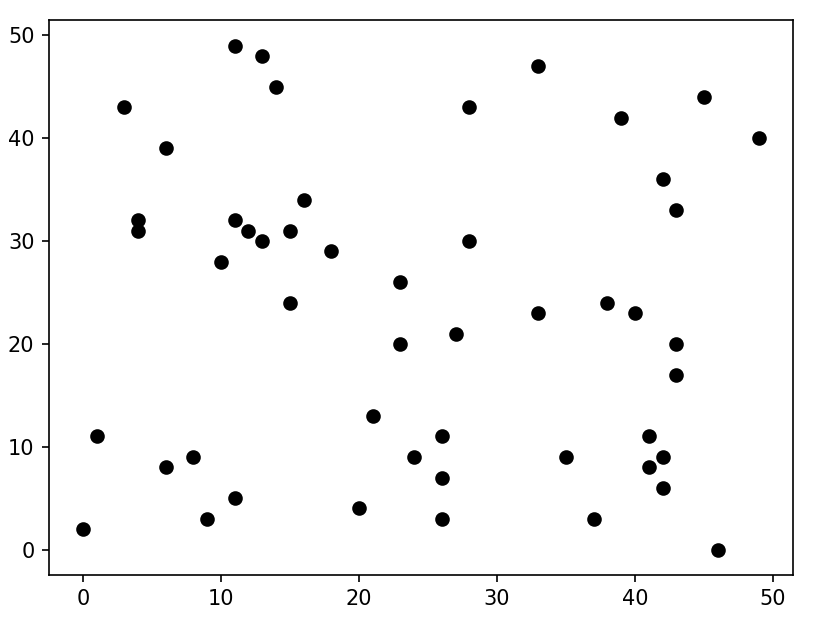
\includegraphics[width = 0.9\textwidth]{imgs/rndpoints.png}
      \captionof{figure}{Initial distribution of random points}
      \label{fig:rndpoints}
  \end{center}

  The first step is to generate an arbitrary number of centroids, i.e. points in space representing the classes to which points will be assigned according to a criterion of maximum closeness.

  \begin{center}
      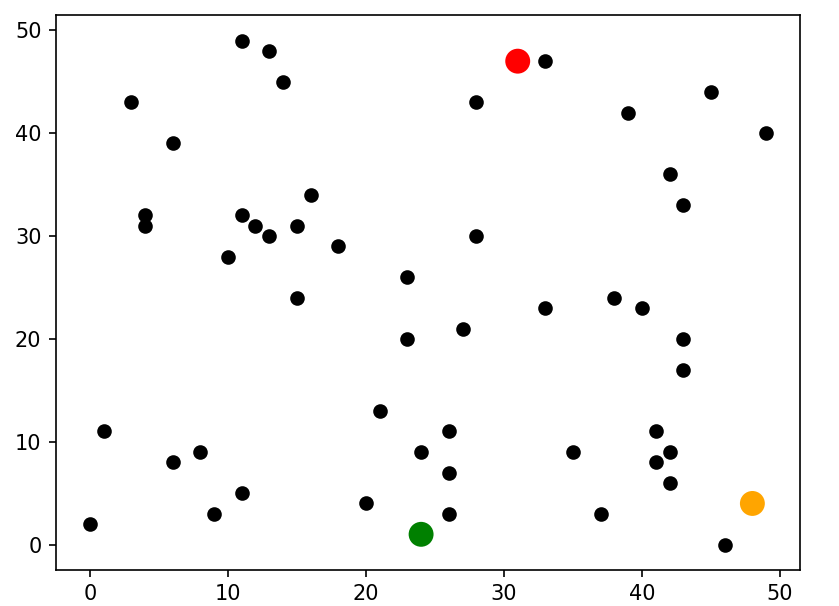
\includegraphics[width = 0.9\textwidth]{imgs/rndcens.png}
      \captionof{figure}{ Random initial position of centroids }
      \label{fig:rndcens}
  \end{center}

  Figure \ref{fig:rndcens} shows three centroids representing 3 classes (red, green, orange). The generation of centroids can be done in 2 ways: by choosing some of the points provided as input, or by randomly generating them in space.

  After that the centroids are generated, each point is assigned a class according to the principle of maximum closeness. 

\end{minipage}
\hspace{0.1in}
\begin{minipage}[b]{0.48\textwidth}
  Given a point P = (x, y) in space its membership class is the one represented by the centroid whose distance from the point is less than that of all other centroids. The choice of how to measure the distance between two points in space affects the final result of the classification. Therefore it is necessary to specify which measure is being used, in this case the Euclidean distance. Given two points A = ($a_x$, $a_y$) and B = ($b_x$, $b_y$) the Euclidean distance is calculated as
  \begin{equation}
      d(A, B) = \sqrt{(a_x - b_x)^2 + (a_y - b_y)^2}
  \end{equation}

  Figure \ref{fig:pointasgn} shows the points after they have been assigned to the closest centroid.

  \begin{center}    
      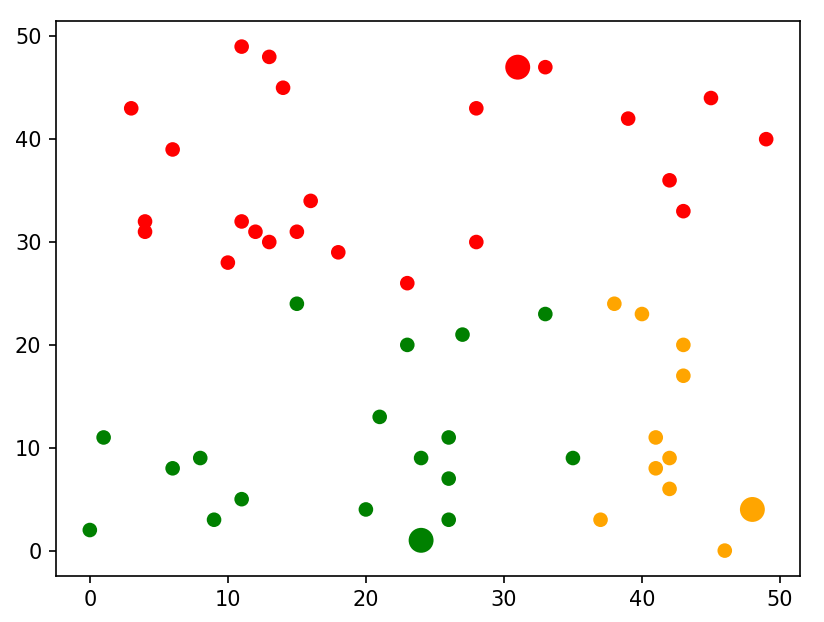
\includegraphics[width = 0.9\textwidth]{imgs/asgnpoints.png}
      \captionof{figure}{Points after the assignation}
      \label{fig:pointasgn}
  \end{center}

  The next step is to reposition the centroids by calculating the average of all points belonging to its class. If $C_i$ is the i-th centroid, its new position ($\tilde{C_i}$) can be calculated as
  \begin{equation}
      \tilde{C_i} = \frac{1}{N_i}\cdot \sum_{p \in C_i} p
      \label{eq:centrep}
  \end{equation}

  Where $N_i$ is the number of points belonging to the i-th class.
  Figure \ref{fig:reccens} shows the centroids after being repositioned. 
  
  \begin{center}    
      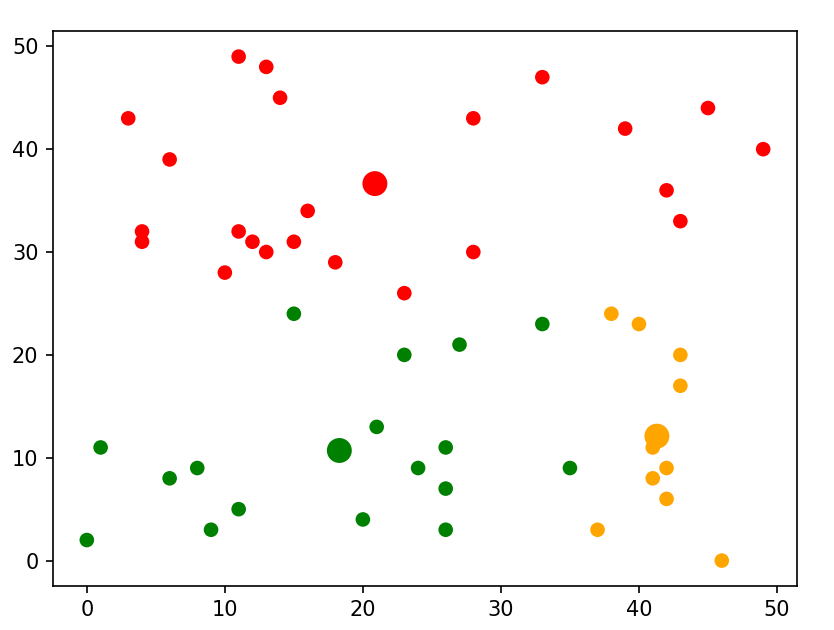
\includegraphics[width = 0.9\textwidth]{imgs/reccens.png}
      \captionof{figure}{Centroids after being recalculated}
      \label{fig:reccens}
  \end{center}

  Now the point assignation is repeated and then the centroid recalculation and so on  until a convergence criterion is reached, which for example could be when the centroids do not shift more than a certain threshold, or simply after a certain number of iterations. This latter method could be usefull when comparing two different algorithm (like lloyd vs hamerly algorithm which is described later)
\end{minipage}

\newpage

\begin{minipage}[b]{0.48\textwidth}
    because the two could converge after a different number of iterations therefore by using a fixed number of repetitions it is easy to compare the result after the same number of cycles. Because of this, for this report, this second approach has been used.

  \section*{Number of iterations}
  The iterations required during a single cycle are \[N\cdot K\cdot d\] where $N$ is the number of points, $K$ is the number of centroids and d is the dimensionality of the data. This is because for each point it is necessary to calculate the distance to each centroid to know which is the least, and to calculate the distance it is necessary to sum k terms (one for each dimension).

  So if m is the number of cycles, the iterations needed are in total
  \begin{equation}
    m(N\cdot K\cdot d)
  \end{equation}

    \begin{algorithm}[H]
        \caption{k-means pseudo-code}\label{alg:cap}
        \begin{algorithmic}
            \State Let "points" be the set of all points
            \State Let "centroids" be the set of all centroids
            \For{ i $<$ iterations }
            \\
            \Comment Point assignation
            \For{ $p$ in points }
                \State mindist = $\min\limits_{j} d(p, C_j)$
                \State old\_centroid = p.centroid\_index
                \State p.centroid\_index = j\\

                \For{l $<$ d}
                    \State coord = p.get\_coord(l)
                    \State average\_per\_class[j][l] += coord

                    \If {old\_centroid $\neq$ -1}
                        \State average\_per\_class[old\_centroid][l] -= coord
                    \EndIf
                \EndFor\\

                \State average\_per\_class[j] += 1
                \If {p.centroid\_index $\neq$ -1}
                    \State average\_per\_class[old\_centroid] -= 1
                \EndIf
            \EndFor
            \\
            \Comment Centroid update

            \For {c in centroids}
                \State nPoints = points\_per\_class[i]
                \For {j $<$ d}
                    \State new\_coord = average\_per\_class[i][j] / nPoints
                    \State c.set\_coord(j, new\_coord)
                \EndFor
            \EndFor
        \EndFor
        \end{algorithmic}
    \end{algorithm}

    \section*{Tracking points belonging to a class}
    During the point assignation step, an important operation is made: tracking which points belong to the classes. In particular we are referring to the following part of the code 
\end{minipage}
\hspace{0.1in}
\begin{minipage}[b]{0.48\textwidth}
    \begin{algorithm}[H]
        \caption{k-means pseudo-code}\label{alg:cap}
        \begin{algorithmic}
            \For{l $<$ d}
                \State coord = p.get\_coord(l)
                \State average\_per\_class[j][l] += coord

                \If {old\_centroid $\neq$ -1}
                    \State average\_per\_class[old\_centroid][l] -= coord
                \EndIf
            \EndFor\\

            \State average\_per\_class[j] += 1
            \If {p.centroid\_index $\neq$ -1}
                \State average\_per\_class[old\_centroid] -= 1
            \EndIf
        \end{algorithmic}
    \end{algorithm}

    Since this is an important process and might not be instantly clear, in this section we will go a little bit deeper and explain how the point tracking is done.

    First of all the average\_per\_class matrix, which is a Kxd matrix that contains, for each row, the sum of all coordinates of the points belonging to that class.

    Then the points\_per\_class array, which is an array with a length of K and, for each class, it contains the number of points which are contained in that class.\\

    Thus, when a point is assigned to the j-th class, its coordinates are added to the average\_per\_class[j] row of the matrix while points\_per\_class[j] is incremented by one.
    It is also important to remove the point from the previous class if it was previously assigned to one. The way to verify it is through the condition $p.centroid\_index != -1$. If the condition is true it means that the points had a previous class. After the verification of the condition, to remove the point from its previous class, its coordinate need to be subtracted from the average\_per\_class[p.centroid\_index] row and points\_per\_class[p.centroid\_index] need to be decremented by one.\\

    Thanks to this process which is done during the points assignation, the following step (i.e. centroid update) is much easier to do. In fact, it is enough to go through the matrix lines and divide it by the total number of points in that class which is contained in the points\_per\_class array.
\end{minipage}

\end{document}